
\documentclass{article}\usepackage[]{graphicx}\usepackage[]{color}
%% maxwidth is the original width if it is less than linewidth
%% otherwise use linewidth (to make sure the graphics do not exceed the margin)
\makeatletter
\def\maxwidth{ %
  \ifdim\Gin@nat@width>\linewidth
    \linewidth
  \else
    \Gin@nat@width
  \fi
}
\makeatother

\definecolor{fgcolor}{rgb}{0.345, 0.345, 0.345}
\newcommand{\hlnum}[1]{\textcolor[rgb]{0.686,0.059,0.569}{#1}}%
\newcommand{\hlstr}[1]{\textcolor[rgb]{0.192,0.494,0.8}{#1}}%
\newcommand{\hlcom}[1]{\textcolor[rgb]{0.678,0.584,0.686}{\textit{#1}}}%
\newcommand{\hlopt}[1]{\textcolor[rgb]{0,0,0}{#1}}%
\newcommand{\hlstd}[1]{\textcolor[rgb]{0.345,0.345,0.345}{#1}}%
\newcommand{\hlkwa}[1]{\textcolor[rgb]{0.161,0.373,0.58}{\textbf{#1}}}%
\newcommand{\hlkwb}[1]{\textcolor[rgb]{0.69,0.353,0.396}{#1}}%
\newcommand{\hlkwc}[1]{\textcolor[rgb]{0.333,0.667,0.333}{#1}}%
\newcommand{\hlkwd}[1]{\textcolor[rgb]{0.737,0.353,0.396}{\textbf{#1}}}%
\let\hlipl\hlkwb

\usepackage{framed}
\makeatletter
\newenvironment{kframe}{%
 \def\at@end@of@kframe{}%
 \ifinner\ifhmode%
  \def\at@end@of@kframe{\end{minipage}}%
  \begin{minipage}{\columnwidth}%
 \fi\fi%
 \def\FrameCommand##1{\hskip\@totalleftmargin \hskip-\fboxsep
 \colorbox{shadecolor}{##1}\hskip-\fboxsep
     % There is no \\@totalrightmargin, so:
     \hskip-\linewidth \hskip-\@totalleftmargin \hskip\columnwidth}%
 \MakeFramed {\advance\hsize-\width
   \@totalleftmargin\z@ \linewidth\hsize
   \@setminipage}}%
 {\par\unskip\endMakeFramed%
 \at@end@of@kframe}
\makeatother

\definecolor{shadecolor}{rgb}{.97, .97, .97}
\definecolor{messagecolor}{rgb}{0, 0, 0}
\definecolor{warningcolor}{rgb}{1, 0, 1}
\definecolor{errorcolor}{rgb}{1, 0, 0}
\newenvironment{knitrout}{}{} % an empty environment to be redefined in TeX

\usepackage{alltt}
\usepackage{graphicx}
\usepackage{hyperref}
\usepackage{amsmath}
\usepackage{times}

\textwidth=6.2in
\textheight=8.5in
%\parskip=.3cm
\oddsidemargin=.1in
\evensidemargin=.1in
\headheight=-.3in


%------------------------------------------------------------
% newcommand
%------------------------------------------------------------
\newcommand{\scscst}{\scriptscriptstyle}
\newcommand{\scst}{\scriptstyle}
\newcommand{\Robject}[1]{{\texttt{#1}}}
\newcommand{\Rfunction}[1]{{\texttt{#1}}}
\newcommand{\Rclass}[1]{\textit{#1}}
\newcommand{\Rpackage}[1]{\textit{#1}}
\newcommand{\Rexpression}[1]{\texttt{#1}}
\newcommand{\Rmethod}[1]{{\texttt{#1}}}
\newcommand{\Rfunarg}[1]{{\texttt{#1}}}
\IfFileExists{upquote.sty}{\usepackage{upquote}}{}
\begin{document}

%------------------------------------------------------------
\title{Simple example of Sweave}
%------------------------------------------------------------
\author{Aedin Culhane}
%\date{}


\maketitle
\tableofcontents


%-------------------------------------------
\section{Introduction}
%--------------------------------------------

Just a simple introduction to Sweave. 

\begin{knitrout}
\definecolor{shadecolor}{rgb}{0.969, 0.969, 0.969}\color{fgcolor}\begin{kframe}
\begin{alltt}
\hlstd{a}\hlkwb{=}\hlnum{1}
\hlstd{b}\hlkwb{=}\hlnum{4}
\hlstd{a}\hlopt{+}\hlstd{b}
\end{alltt}
\begin{verbatim}
## [1] 5
\end{verbatim}
\begin{alltt}
\hlkwd{print}\hlstd{(}\hlstr{"hello"}\hlstd{)}
\end{alltt}
\begin{verbatim}
## [1] "hello"
\end{verbatim}
\end{kframe}
\end{knitrout}

We can call R commands from the text. For example a+b= 5

%-------------------------------------------
\section{Including a Plot}
%--------------------------------------------
Now for a plot.  Note we include fig=TRUE, which prints the plot within the document


\begin{knitrout}
\definecolor{shadecolor}{rgb}{0.969, 0.969, 0.969}\color{fgcolor}\begin{kframe}
\begin{alltt}
\hlkwd{plot}\hlstd{(}\hlnum{1}\hlopt{:}\hlnum{10}\hlstd{,} \hlkwc{col}\hlstd{=}\hlstr{"red"}\hlstd{,} \hlkwc{pch}\hlstd{=}\hlnum{19}\hlstd{)}
\end{alltt}
\end{kframe}
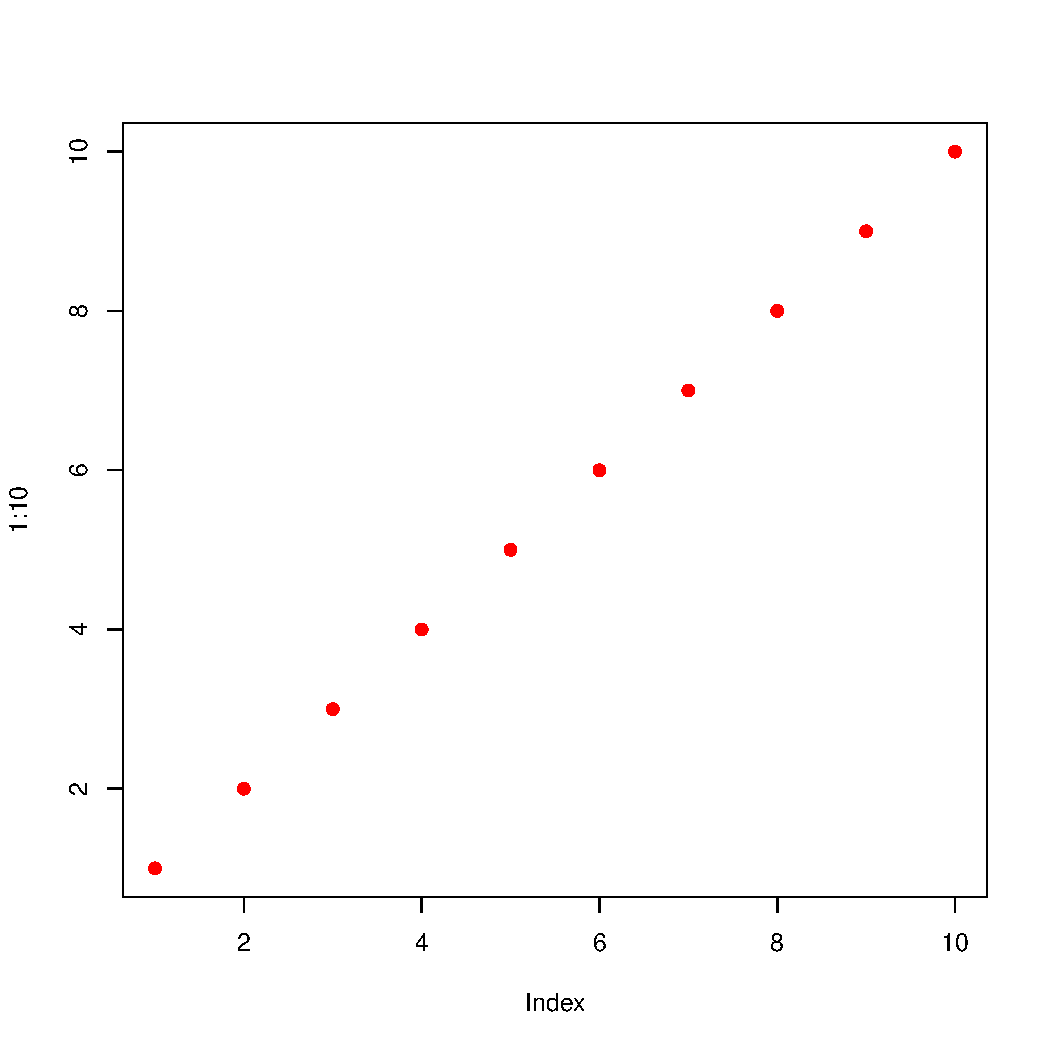
\includegraphics[width=\maxwidth]{figure/test2-1} 

\end{knitrout}

Thats it.... simple hey!


%------------------------------------
\subsection{More on Plots}
%-------------------------------------

To make the plot a little nicer, we can add a caption. Also lets change the size of the plot to be 4" in height and 6" in width

\begin{figure}
\begin{knitrout}
\definecolor{shadecolor}{rgb}{0.969, 0.969, 0.969}\color{fgcolor}\begin{kframe}
\begin{alltt}
\hlkwd{par}\hlstd{(}\hlkwc{mfrow}\hlstd{=}\hlkwd{c}\hlstd{(}\hlnum{1}\hlstd{,}\hlnum{2}\hlstd{))}
\hlkwd{plot}\hlstd{(}\hlnum{1}\hlopt{:}\hlnum{10}\hlstd{,} \hlkwc{col}\hlstd{=}\hlstr{"green"}\hlstd{,} \hlkwc{pch}\hlstd{=}\hlnum{21}\hlstd{)}
\hlkwd{barplot}\hlstd{(}\hlkwc{height}\hlstd{=}\hlkwd{sample}\hlstd{(}\hlnum{1}\hlopt{:}\hlnum{10}\hlstd{,}\hlnum{5}\hlstd{),} \hlkwc{names}\hlstd{=LETTERS[}\hlnum{1}\hlopt{:}\hlnum{5}\hlstd{],} \hlkwc{col}\hlstd{=}\hlnum{1}\hlopt{:}\hlnum{5}\hlstd{)}
\end{alltt}
\end{kframe}
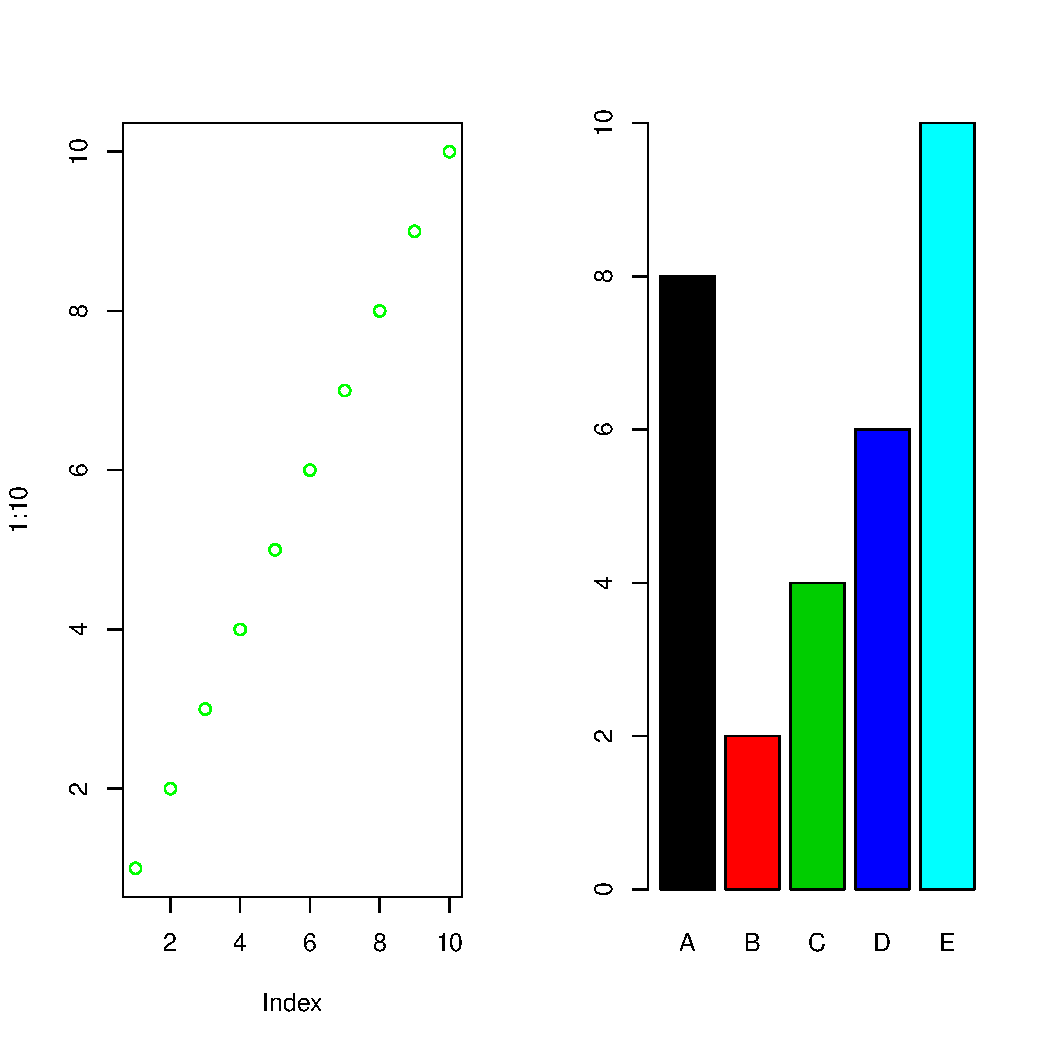
\includegraphics[width=\maxwidth]{figure/test3-1} 

\end{knitrout}

\caption{Plot of 1:10 and a bar plot beside it in a figure that is 4x6 inches}

\end{figure}

\newpage
%------------------------------------
\subsection{Creating a table}
%-------------------------------------

Lets include a table using the dataset,  which is included in the default core installation of R. It contains the height and weight of 15 women.

\begin{knitrout}
\definecolor{shadecolor}{rgb}{0.969, 0.969, 0.969}\color{fgcolor}\begin{kframe}
\begin{alltt}
\hlkwd{require}\hlstd{(xtable)}
\end{alltt}


{\ttfamily\noindent\itshape\color{messagecolor}{\#\# Loading required package: xtable}}\begin{alltt}
\hlstd{myTable}\hlkwb{<-}\hlkwd{summary}\hlstd{(women)}
\end{alltt}
\end{kframe}
\end{knitrout}

We can manually encode a table in latex 


\begin{center}
\begin{tabular}{rrrrrrrr} 

\begin{knitrout}
\definecolor{shadecolor}{rgb}{0.969, 0.969, 0.969}\color{fgcolor}\begin{kframe}
\begin{verbatim}
## $ Min.   :58.0   $&$ Min.   :115.0   $\\
## $ 1st Qu.:61.5   $&$ 1st Qu.:124.5   $\\
## $ Median :65.0   $&$ Median :135.0   $\\
## $ Mean   :65.0   $&$ Mean   :136.7   $\\
## $ 3rd Qu.:68.5   $&$ 3rd Qu.:148.0   $\\
## $ Max.   :72.0   $&$ Max.   :164.0   $\\
\end{verbatim}
\end{kframe}
\end{knitrout}
\end{tabular}
\end{center}

But it is much easier to use the package \Rpackage{xtable}. We use the function \Rfunction{require} to load the package.

\begin{knitrout}
\definecolor{shadecolor}{rgb}{0.969, 0.969, 0.969}\color{fgcolor}\begin{kframe}
\begin{alltt}
\hlstd{xtab}\hlkwb{<-}\hlkwd{xtable}\hlstd{(myTable)}
\hlkwd{print}\hlstd{(xtab,} \hlkwc{floating}\hlstd{=}\hlnum{FALSE}\hlstd{)}
\end{alltt}
\begin{verbatim}
## % latex table generated in R 3.5.1 by xtable 1.8-3 package
## % Wed Oct 17 13:06:22 2018
## \begin{tabular}{rll}
##   \hline
##  &     height &     weight \\ 
##   \hline
## X & Min.   :58.0   & Min.   :115.0   \\ 
##   X.1 & 1st Qu.:61.5   & 1st Qu.:124.5   \\ 
##   X.2 & Median :65.0   & Median :135.0   \\ 
##   X.3 & Mean   :65.0   & Mean   :136.7   \\ 
##   X.4 & 3rd Qu.:68.5   & 3rd Qu.:148.0   \\ 
##   X.5 & Max.   :72.0   & Max.   :164.0   \\ 
##    \hline
## \end{tabular}
\end{verbatim}
\end{kframe}
\end{knitrout}


%------------------------------------
\subsection{More on tables}
%-------------------------------------

Let make the table nice.  Lets exclude the row numbers and include a caption on the table. We can also tag the table so we reference Table~\ref{Table:women} in the text


\begin{knitrout}
\definecolor{shadecolor}{rgb}{0.969, 0.969, 0.969}\color{fgcolor}\begin{kframe}
\begin{alltt}
\hlstd{xtab2}\hlkwb{<-}\hlkwd{xtable}\hlstd{(myTable,} \hlkwc{caption}\hlstd{=}\hlstr{"Summary of women data"}\hlstd{,}  \hlkwc{label}\hlstd{=}\hlstr{"Table:women"}\hlstd{)}
\hlkwd{print}\hlstd{(xtab2,}\hlkwc{include.rownames} \hlstd{=} \hlnum{FALSE}\hlstd{)}
\end{alltt}
\begin{verbatim}
## % latex table generated in R 3.5.1 by xtable 1.8-3 package
## % Wed Oct 17 13:06:22 2018
## \begin{table}[ht]
## \centering
## \begin{tabular}{ll}
##   \hline
##     height &     weight \\ 
##   \hline
## Min.   :58.0   & Min.   :115.0   \\ 
##   1st Qu.:61.5   & 1st Qu.:124.5   \\ 
##   Median :65.0   & Median :135.0   \\ 
##   Mean   :65.0   & Mean   :136.7   \\ 
##   3rd Qu.:68.5   & 3rd Qu.:148.0   \\ 
##   Max.   :72.0   & Max.   :164.0   \\ 
##    \hline
## \end{tabular}
## \caption{Summary of women data} 
## \label{Table:women}
## \end{table}
\end{verbatim}
\end{kframe}
\end{knitrout}

\newpage
%------------------------------------
%handy to include this at the end
%------------------------------------
\section{SessionInfo}
%-------------------------------------

\begin{knitrout}
\definecolor{shadecolor}{rgb}{0.969, 0.969, 0.969}\color{fgcolor}\begin{kframe}
\begin{alltt}
\hlkwd{sessionInfo}\hlstd{();}
\end{alltt}
\begin{verbatim}
## R version 3.5.1 (2018-07-02)
## Platform: x86_64-w64-mingw32/x64 (64-bit)
## Running under: Windows 10 x64 (build 17134)
## 
## Matrix products: default
## 
## locale:
## [1] LC_COLLATE=German_Germany.1252  LC_CTYPE=German_Germany.1252   
## [3] LC_MONETARY=German_Germany.1252 LC_NUMERIC=C                   
## [5] LC_TIME=German_Germany.1252    
## 
## attached base packages:
## [1] stats     graphics  grDevices utils     datasets  methods   base     
## 
## other attached packages:
## [1] xtable_1.8-3 knitr_1.20  
## 
## loaded via a namespace (and not attached):
## [1] compiler_3.5.1 magrittr_1.5   tools_3.5.1    stringi_1.1.7 
## [5] highr_0.7      stringr_1.3.1  evaluate_0.11
\end{verbatim}
\end{kframe}
\end{knitrout}

\end{document}
